\chapter{Physical Object Reconstruction}\label{ch:reco}

Physical properties of particles produced from a collision at the \ac{lhc} are derived by combining the traces and deposits these particles leave in the various subdetectors as they traverse \ac{atlas}. The upcoming sections will describe the reconstruction processes for various objects used in this analysis. The primary reference for this chapter is \citep{atlas2021optimisation}.

\section{Tracks and Primary Vertex}\label{sec:tracks}
Charged particles leave a trajectory in the \ac{id} as explained in section \ref{sec:inner_detector}. To reconstruct the path of these particles an algorithm first groups hits that are close to each other in the silicon detectors into clusters. These clusters are then successively combined to determine the most probable trajectory that the particles have taken through the detector which are referred to as tracks \citep{aaboud2017performance}. These are then geometrically matched to proton-proton interactions and the vertex with the largest scalar sum of transverse momenta $\sum \pt^2$ is identified as the primary hard scatter vertex if at least two tracks with $\pt>\qty[]{500}{MeV}$ are in the tracking volume $\abs{\eta}<2.5$. The momentum of particles is inferred from the curvature caused by the magnetic field.

\section{Jets}\label{sec:jets}
As discussed in section \ref{sec:renormalization} quarks cannot be observed individually but only as colorless hadrons. When decaying they undergo showering and hadronization forming cone-like structures of energy deposits in the detector called jets. They are reconstructed by combining and grouping both \ac{id} and calorimeter information.

\subsection{Topo-Cluster}
As outlined in section \ref{sec:calorimeters}, decaying particles deposit energy in the calorimeters. These energy deposits are three-dimensionally grouped by topologically connected calorimeter cells into structures known as Topo-Clusters. The formation of these clusters begins with cells that exhibit signals exceeding four times the standard deviation of the detector noise ($4\sigma_\mathrm{noise}$). These cells act as seeds to form a Topo-Cluster if they are surrounded by cells with signals above two times the noise level ($2\sigma_\mathrm{noise}$).

\subsection{Particle Flow Object}\label{sec:particle_flow}
The energy and mass resolution calculated from Topo-Clusters can be improved by geometrically matching tracks to the clusters. This exploits the superior momentum and position resolution of the \ac{id} compared to the calorimeters to complement the energy measurements obtained from the calorimeter. When a track is successfully matched to a Topo-Cluster, the expected energy, based on the particle that created the track, is computed. From this expected energy all associated cluster cell energies are subtracted and the remnant is removed from the expected energy if energy is within the range of typical fluctuations. Such combination of a Topo-Cluster and a track are called \ac{pfo} \citep{aaboud2017jet}. Sometimes the energy of one track ends up in several clusters. For this the Particle Flow algorithm combines the most probable clusters with the track. Topo-Clusters without matched tracks are assumed to be neutral particles as they do not leave a trace in the \ac{id}. \acp{pfo} not matched to the \ac{pv} are removed to reduce the contribution from pileup.  This technique, especially in the reconstruction of low \pt clusters, enhances the overall resolution.

\subsection{Track-CaloClusters}
Instead of using the energy measurement of the tracks as for \acp{pfo} for \acp{tcc} the calorimeter energy measurement is used and complemented by the angular information of the tracks. \ac{tcc} was developed for high \pt jets since the resolution in the calorimeters improves with larger momentum when calorimeter deposits become more localized. The procedure involves two steps. High quality tracks are selected and extrapolated to the Topo-Clusters. If the extrapolation uncertainty exceeds the Topo-Cluster width the tracks is removed. If a track-cluster pair is found it will only be accepted if their angular separation is smaller than the quadratically summed Topo-Cluster width and track extrapolation uncertainty $\Delta R < \sqrt{\sigma_\text{cluster}^2+\sigma_\text{track}^2}$ \citep{ATL-PHYS-PUB-2017-015}.

\subsection{Unified Flow Object}
\acp{pfo} benefit from better momentum/energy resolution of the \ac{id} compared to the calorimeters at low momenta. However, as momentum and particle density increase, the process of matching tracks to clusters becomes increasingly ambiguous. To address this issue the Topo-Clusters used in the particle flow algorithm are refined with \acp{tcc} which produces \acp{ufo}. This method allows the algorithm to select the most effective reconstruction technique for the given conditions \citep{atlas2021optimisation,ATL-PHYS-PUB-2022-038}.


\subsection{Jet Clustering Algorithm}\label{sec:anti_kt}
The definition of a jet is not unique as it depends on the size and direction of the cone and thus how many particles are included. For this the Anti-$k_t$ algorithm \citep{cacciari2008anti} clusters aforementioned four vector objects in this section into cone-shaped jets. It starts with calculating the distances between all four vector objects $i,j$ that are considered
\begin{equation}
  d_{ij}=\frac{1}{\max(p_{T,i}^{2}\,,\,p_{T,j}^{2})} \frac{\Delta R_{ij}^2}{R^2},
\end{equation}
and the distance to the beam
\begin{equation}
  d_{iB}=\frac{1}{p_{T,i}^{2}},
\end{equation}
with the transverse momenta of the particles $p_{T,i},p_{T,j}$ their angular distance $\Delta R$ as of equation \ref{eq:delta_R} and a chosen radius parameter $R$. The algorithm combines objects $i,j$ into a new four vector for the smallest distance $d_{ij}$. The distance is small for large transverse momenta \pt and small angular distances $\Delta R_{ij}$ and are therefore preferred by the algorithm. After combining two objects the algorithm runs as long as $d_{iB}<d_{ij}$. Thus it stops once particles outside of the chosen radius would be added. In \ac{atlas} jets with a radius parameter of $R=0.4 (1.0)$ are denoted as Small-R(Large-R) jets. If the first factor of $d_{i,j}$ is exchanged to $\min(p_{T,i}^{2}\,,\,p_{T,j}^{2})$ the algorithm is called $k_t$ and the Cambridge/Aachen version is $\min(p_{T,i}\,,\,p_{T,j})$.


% \subsection{Variable Radius Jets}\label{sec:vr_jets}
% In very boosted regimes mit large momenta individual jets can overlap. In order to still reconstruct them individually a \ac{vr} for the $R$ parameter from the Anti-$k_t$ Jet Clustering Algorithm of section \ref{sec:anti_kt} is used
% \begin{equation}
%   R\rightarrow R_\text{eff}(\pt)=\frac{\rho}{\pt}
% \end{equation}
% It becomes therefore dependent on the transverse momentum and is controlled by a parameter $\rho$ so that the jet size decreases with \pt. \ac{vr} jets are reconstructed from tracks and are required to have $\pt>\qty[]{10}{GeV}$.

\section{$b$-tagging}\label{sec:b_tagging}
This analysis has four $b$-quarks in the final state and therefore relies on their identification. One of the key characteristics of $b$ quarks is their relatively large mass resulting in a long lifetime compared to other quarks $\tau\sim\qty{1.5}{ps}$. This translates to a decay length of about $c\tau \sim \qty{450}{\micro m}$ and leads to a secondary vertex. Although these $b$-hadrons do not reach the \ac{id} directly their decay positions can be deduced from tracks.

Such tracks have a large impact parameter that is defined as the distance of closest approach in the $r-\phi$ projection in transverse $d_0$ and longitudinal $z_o$ direction \citep{aad2008atlas} as illustrated in figure \ref{fig:secondary_vertex}b. Other methods for determining the secondary vertex attempt to connect the tracks of the $b$-hadron decay with those of a subsequent $c$-hadron decay by aligning the tracks in Fig. \ref{fig:secondary_vertex}a and also by deriving the mutual origins of the tracks \citep{ATL-PHYS-PUB-2017-013}.
\begin{figure}[]
  \centering
  \subfigure[]{
    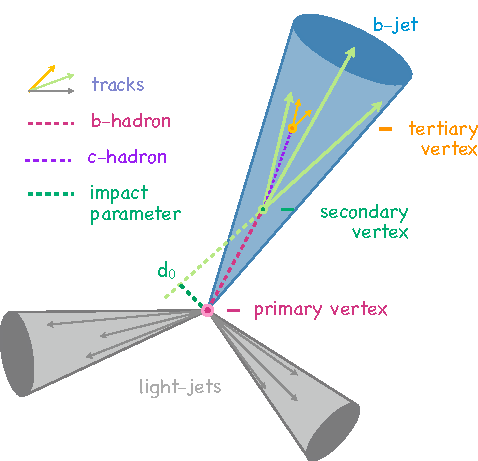
\includegraphics[width=0.49\textwidth]{secVexMguth}
  }%\hspace*{1cm}
  \subfigure[]{
    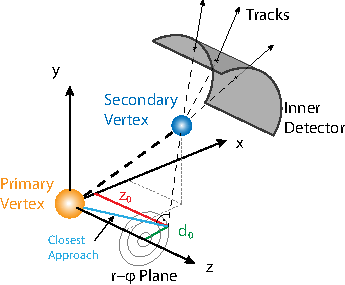
\includegraphics[width=0.49\textwidth]{SV_sketch}
  }
  \caption{(a) Example decay of a $b$-hadron (\hexbox{8AB2D3}) and jets from light flavor hadrons (\hexbox{C5C6C6}) (Adopted from \cite{Guth:2765038}). (b) Impact parameters defined for tracks as distance of closest approach to the primary vertex in the $r-\phi$-plane (\mbox{\color[HTML]{009245}{$d_0$}}) and along the z axis (\mbox{\color[HTML]{EC1C25}{$z_0$}}).}
  \label{fig:secondary_vertex}
\end{figure}

\subsection{DL1d Tagger}
The results obtained from the secondary vertex- and impact parameter finding algorithms by exploiting the characteristics of $b$-hadron decays and the kinematics of the jet are then passed into a deep feed-forward neural network called DL1d which is trained to distinguish $b$-jets from jets of other flavors \citep{atlas2022atlas}. The output nodes for flavor classification ($p_\mathrm{b}, p_\mathrm{c}, p_\mathrm{light}$) are further combined into a single discriminating score variable
\begin{equation}
  D_\mathrm{DL1d}=\ln\left(\frac{p_b}{f_c \cdot p_c + (1-f_c)\cdot p_\mathrm{light} }\right).
\end{equation}
$f_c$ is a parameter to tune the importance between charm and light quark background classes ($\sum f_\mathrm{bkg} =1$). When evaluating the \ac{nn} a value for the discriminating variable $D$ can be derived that corresponds to a $b$-jet selection efficiency. In this analysis the chosen efficiency is \qty[]{77}{\percent}. 

\subsection{GN2X Tagger}\label{sec:gn2x}
For a collision event with decay products consisting of two $b$-jets with large transverse momenta, small-$R=$ jets can become overlapped making a clear separation infeasible. To address such scenarios, large-$R$ jets are used that encompass both $b$-jets. The latest iteration of $b$-tagging algorithms in \ac{atlas} uses \acp{gnn} \citep{shlomi2020graph, ATL-PHYS-PUB-2022-027}. This choice is such that a graph with edges and vertices represents a more natural relational structure of a jet opposed to a feed-forward \ac{nn}. This involves globally updated states on all network parameters, modeling the properties of the whole jet, e.g. its flavor origin, as well as tracks as vertices and their interactions as edges between them. 

The GN2X tagger uses a transformer architecture \citep{ATL-PHYS-PUB-2023-021} within a \ac{gnn}. Transformers are able to capture the relationships between sequential objects, a feature present in particle decays. The input features to this model include the transverse momentum ($p_T$), pseudorapidity ($\eta$), and mass of the jet, along with properties of tracks associated with the jet. It aims to identify the quark content in potential Higgs boson decays by outputting probabilities for the decays into two $b$-quarks, two $c$-quarks, a top quark, and contributions from multijet background processes. The GN2X tagger then computes a discriminant, based on these probabilities:
\begin{equation}
  D_{\text{GN2X}}=\ln\left({\frac{p_{\text{Hbb}}}{
    f_{\text{Hcc}}\cdot p_{\text{Hcc}}+
    f_{\text{top}}\cdot p_{\text{top}}+
    (1-f_{\text{Hcc}}-f_{\text{top}})\cdot p_{\text{QCD}}}}\right).
\end{equation}
$f_\text{top}=0.25$ and $f_\text{Hcc}=0.02$ denotes chosen parameters weighting the influence of the corresponding \ac{gnn} output nodes to the discriminant. From the evaluation of the discriminant \acp{wp} are defined depending on the Higgs tagging efficiency. As mentioned in \citep{ATL-PHYS-PUB-2023-021} mass sculpting is observed which can become a problem for a data-driven background estimate as used in this thesis. This issue has been addressed by slightly altering the discriminant value depending on the mass of the jet in a way that the \ac{qcd} background selection efficiency is not altered by the tagger. 

% The $X\rightarrow bb$ tagger is a feed-forward \ac{nn} \citep{ATL-PHYS-PUB-2020-019}. The inputs include the transverse momentum \pt and pseudorapidity $\eta$ of the large-$R$ jet along with outputs from DL1d for up to three \ac{vr} track jets. Similar to DL1d, a discriminant is computed from the \ac{nn}'s output scores, which reflect the likelihood of the event being a Higgs, top, or multijet decay:
% \begin{equation}
%   D_{\text{Xbb}}=\ln\left({\frac{p_{\text{Higgs}}}{f_{\text{top}}\cdot p_{\text{top}}+(1-f_{\text{top}})\cdot p_{\text{multijet}}}}\right).
% \end{equation}
% $f_\text{top}$ denotes the top fraction with regards to the multijet output. From the evaluation of the discriminant \acp{wp} are defined depending on the Higgs tagging efficiency.

\section{Jet Calibration}\label{sec:calibration}
The calibration of measuring instruments is crucial for accuracy, and this is especially true for the reconstruction of jets. The following factors often lead to discrepancies between the reconstructed and actual properties of jets \citep{atlas2011jet}:
\begin{itemize}
\item \textbf{Non-Compensation:} A lower calorimeter response to non-electromagnetic particles from hadron showers compared to electromagnetic particles.
\item \textbf{Dead Material:} Energy is deposited in non-instrumented areas of the detector.
\item \textbf{Out-of-Cone Particles:} Particles from a decay are not captured within the jet reconstruction cone.
\item \textbf{Noise Threshold:} Energy depositions below the detector's noise threshold are missed.
\item \textbf{Pile-up:} Additional particles from other proton-proton interactions. 
\item \textbf{Leakage:} Particles are not stopped inside the calorimeter (punch-through).
\end{itemize}
Several algorithms are employed to mitigate these effects and to also take the detector geometry into account and are described in the following based on \citep{atlas2021jet}. As reference objects serve well-understood physics processes that leave a distinct signature in the detector like dijet events or decays of $Z$-bosons or photons.

\subsection{Pile-up Mitigation}
When bunches of protons are collided, not only one but rather several proton-proton interactions are measured. Various methods have been developed to isolate interactions and are described for both small and large $R$ jets. The mean number of interactions is commonly referred to as pile-up and is categorized into in-time pile-up referring to additional proton-proton collisions occurring within the same bunch-crossing and out-of-time pile-up collisions occurring before and after the collision of interest. Over time these methods have seen significant improvements allowing to record and disentangle more collision events per bunch crossing. This increase in pile-up during the data taking period is depicted in Figure \ref{fig:pileup}.
\begin{figure}
  \centering
  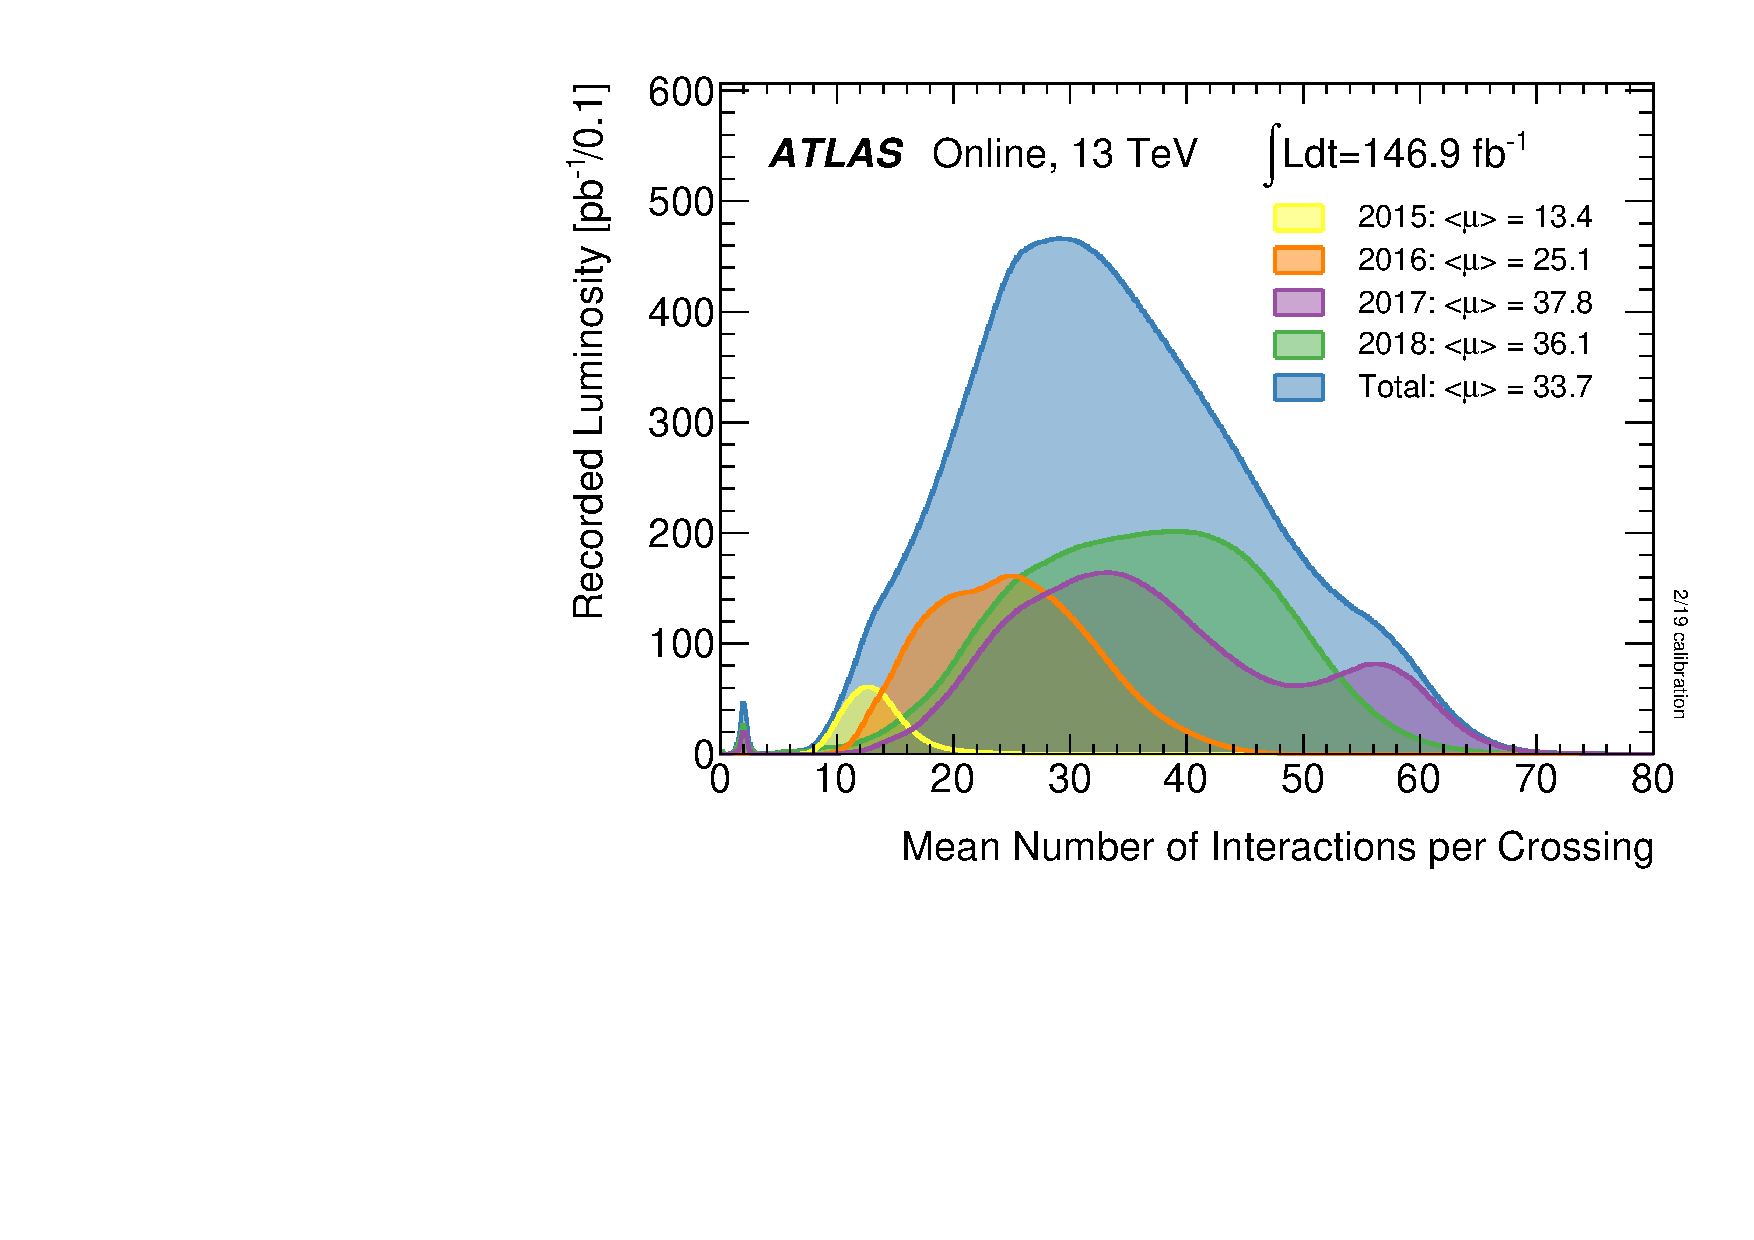
\includegraphics[width=0.5\textwidth]{mu_2015_2018}
  \caption[]{Pile up profiles for run 2 data taking periods \citep{pileup}.}
  \label{fig:pileup}
\end{figure}


\subsubsection{Small-R Jets}
At a first step contributions from pileup are reduced by subtracting the median transverse momentum density $\rho=\pt / A$ of $k_t$-reclustered jets found within $\eta<2.0$ multiplied by the area of the jet $A_T$. This area is determined by uniformly adding massless `ghost' particles to the event. The area in $(\eta-\phi)$ space covered by ghosts clustered to a jet determine its area \citep{ATLAS-CONF-2017-065}. Another reduction observes that the pileup corrected \pt is a function of the number of primary Vertices $N_\text{PV}$ and the mean number of interactions $\mu$. Thus the corrected transverse momentum is expressed as
\begin{equation}
  \pt^\text{corr}=\pt-\rho A_T -\alpha(N_\text{PV}-1)-\beta\mu
\end{equation}
with parameters $\alpha$ and $\beta$. The effect of the correction is shown in figure \ref{fig:jet_pt_correction}.
\begin{figure}
  \centering
  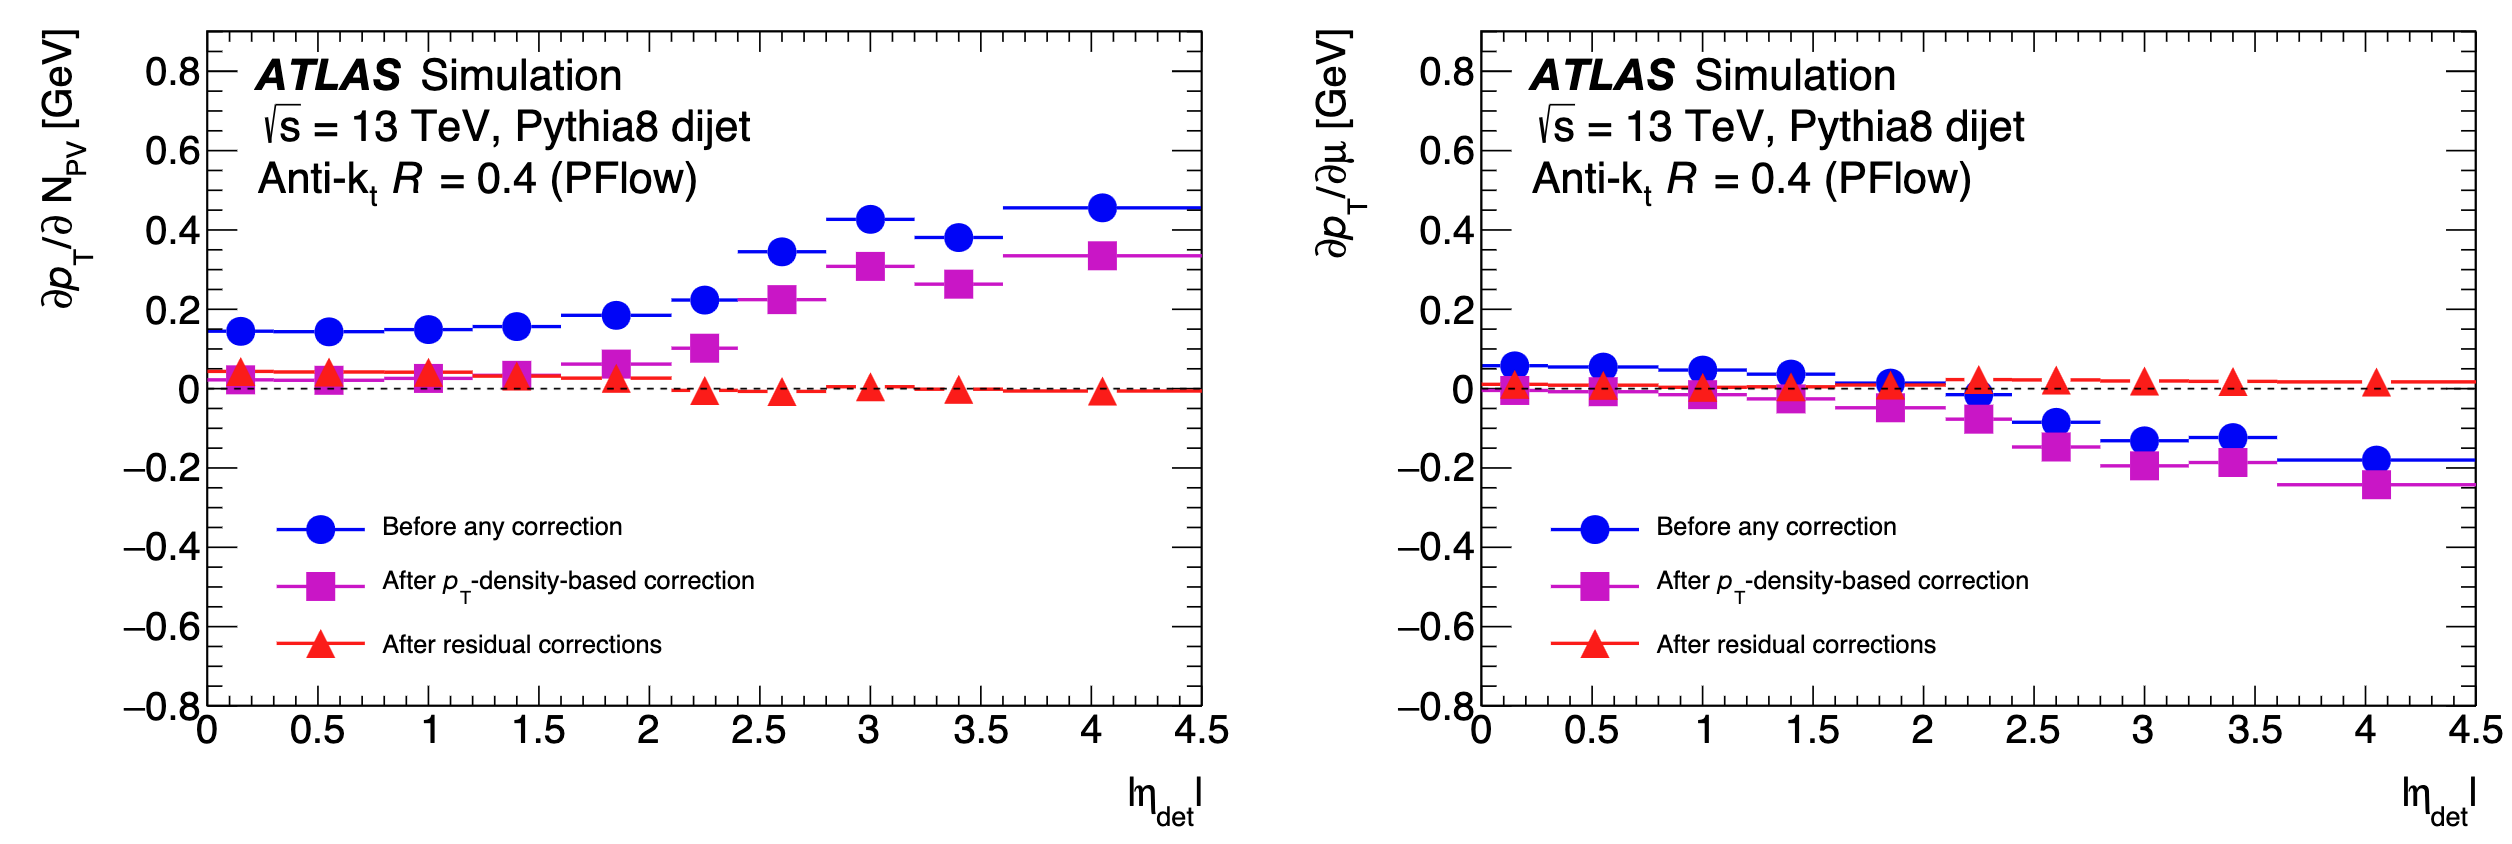
\includegraphics[width=1\textwidth]{jet_pt_correction}
  \caption[]{\pt correction to remove the \pt dependence of the jet at different $\eta$ for: (left)\pt dependent on the number of primary vertices and (right) average number of interactions of the collision.}
  \label{fig:jet_pt_correction}
\end{figure}

Moreover pileup contributions can be further reduced by comparing the scalar \pt sum of tracks from the \ac{pv} associated to the jet with the scalar \pt sum of all tracks including other \acp{pv}. The \ac{jvt} \citep{ATLAS-CONF-2014-018} uses this property to apply a quality criterion on jets with $\pt<\qty[]{60}{GeV}$ and $|\eta|<2.4$.


\subsubsection{Large-R Jets}
Due to their large surface area, large-$R$ jets are particularly susceptible to pile-up contributions. Several algorithms are used to mitigate it \citep{atlas2021optimisation}. Similar to the median \pt subtraction for small-$R$ jets a so-called constituent subtraction (CS) is applied. In this method, a pile-up estimate per ghost particle is iteratively subtracted from the clusters that are closest to the ghosts in the jet \citep{ATLAS-CONF-2017-065}. 

Additionally, an algorithm named SoftKiller (SK) imposes a \pt requirement on constituents to eliminate soft particles. This \pt-cut is determined per event by selecting a \pt-value that leaves half of the cells in an ($\eta,\phi$) grid empty, effectively achieving a median \pt of zero, akin to that used in constituent subtraction \citep{ATLAS-CONF-2017-065}.

Another method employed is jet grooming, which aims to remove low energy (soft) wide-angle radiation from the jet. This is achieved through the SoftDrop (SD) algorithm, which applies the Cambridge/Aachen clustering method \citep{Larkoski_2014}. This clustering approach groups the jet's constituents based on their angular distance. Recursively a \pt requirement is applied to constituents always checked on the widest angle constituent with a stopping criterion. 

% This series of strategies ensures a more accurate reconstruction of jets


% In this process, a large $R$-jet is divided into smaller sub-jets with a radius of $R=0.2$. Of these subjets, only those that contain at least $\pt>\qty[]{5}{\percent}$ of the original large-$R$ jet are retained.



\subsection{\ac{jes}, $\eta$ and Mass}
\begin{figure}
  \centering
  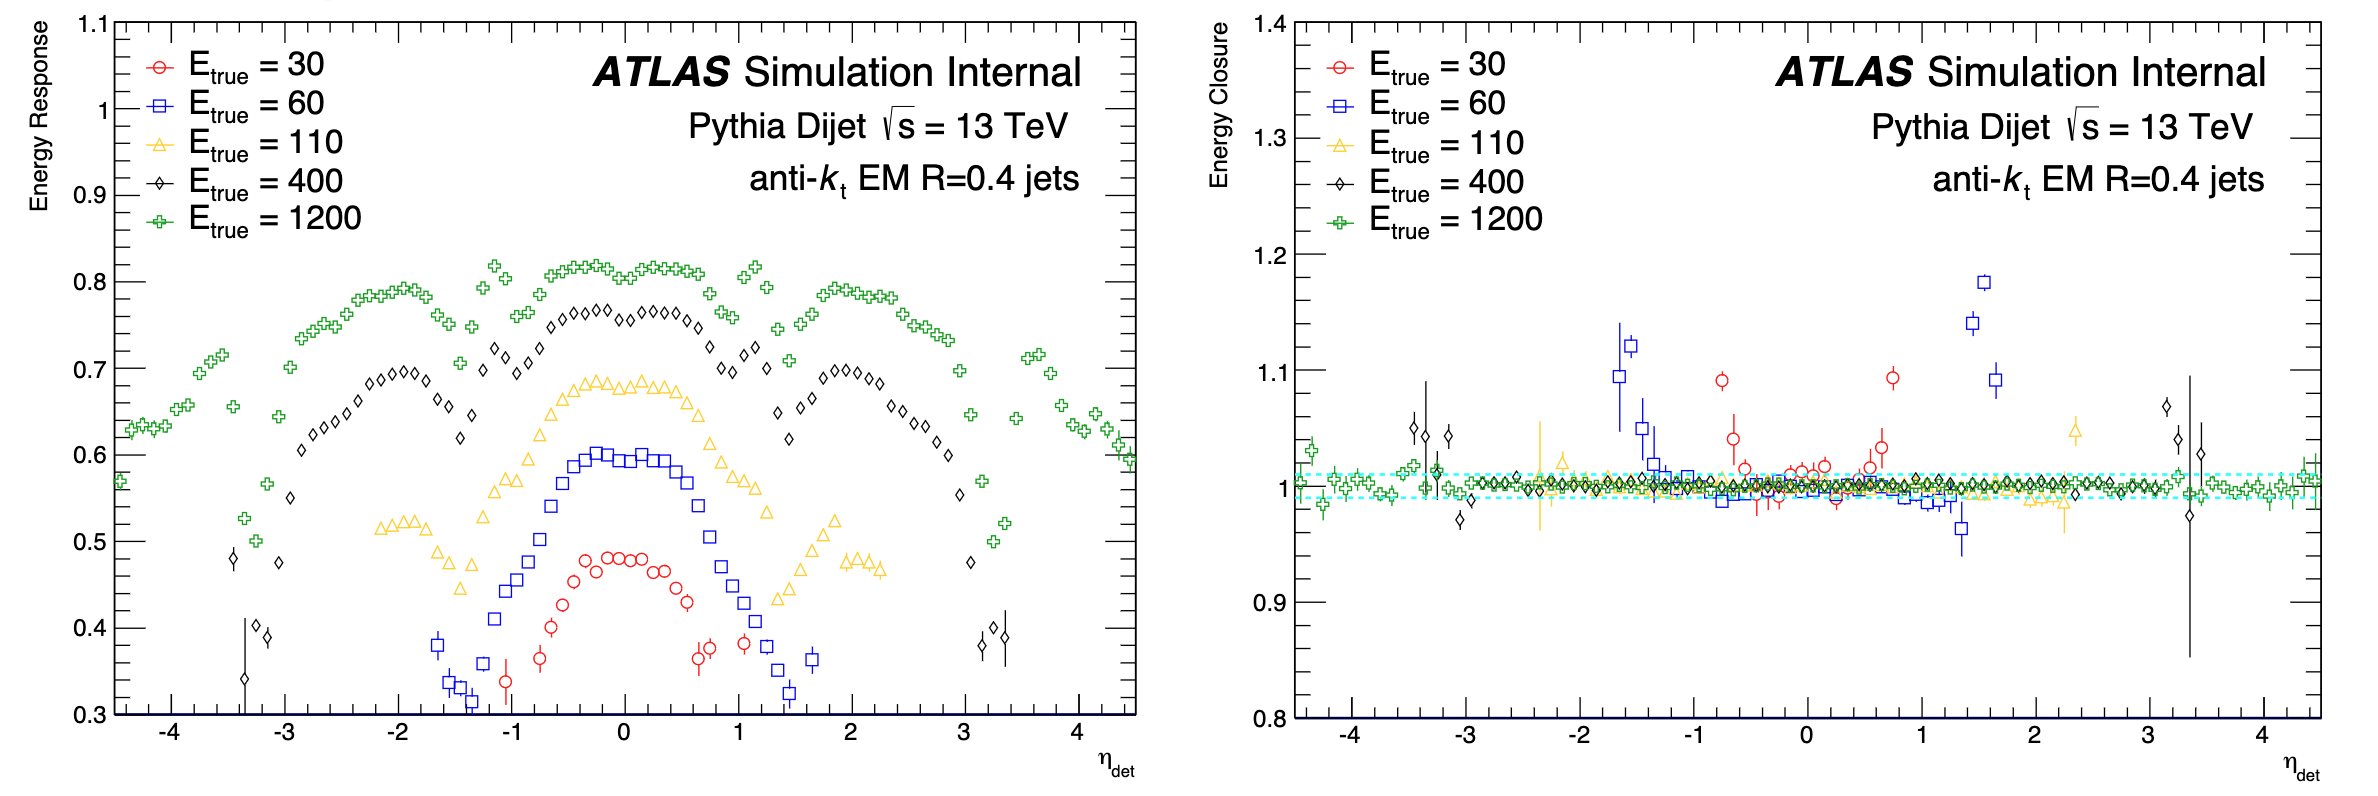
\includegraphics[width=1\textwidth]{jet_eta_mismatch}
  \caption[]{Jet energy response $E_\text{reco}/E_\text{truth}$ for different detector $\eta$ values (left) before and after applying (right) the calibration. Adopted from \citep{jet_eta_calib}.}
  \label{fig:jet_eta_mismatch}
\end{figure}
Figure \ref{fig:jet_eta_mismatch} depicts a mismatch between reconstructed and truth energy of simulated two jet events measured in $\eta$ bins. Based on this observation a continuous correction function in $\eta$ is derived and applied to correct for differences in jet energy, $\eta$ and mass \citep{atlas2011jet,Aaboud:2019aa}. This is exemplified in the right hand plot of figure \ref{fig:jet_eta_mismatch}.

\subsection{Global Sequential Calibration}
This step corrects the jet \pt without changing the mean energy of the jet. It corrects for non-compensation, dead material and leakage effects by using observables like the charged particle fraction, energy fractions in different calorimeter layers, track-related quantities and the muon activity behind the calorimeter. Corrections are again derived in \pt and $\eta$ and are applied sequentially.

\subsection{In Situ Calibration}
In the final calibration step, discrepancies between actual data and simulations are corrected in terms of transverse momentum \pt. These discrepancies arise from the imperfect simulation of detector materials and inaccuracies in modeling the underlying physics processes involved. To address these issues, well-established physics processes are used as benchmarks, and from these, correction factors in \pt are derived. This step is only applied to data.

\subsection{Jet Event Cleaning}
Another method to reduce background is called event cleaning. It removes the whole event if jets are found that where generated by out-of-time pileup, cosmic rays or beam-induced backgrounds by applying a set of quality criteria to variables describing the jet profile \citep{ATLAS-CONF-2015-029}.

\subsection{Mass Correction For Large-$R$ Jets}
The mass of a jet is calculated from the energy deposits in calorimeter clusters $i$ via
\begin{equation}
  m_{\text{calo}} = \sqrt{\left(\sum_{i\in \text{Jet}}E_i\right)^2-\left(\sum_{i\in \text{Jet}}\vec{p_i}\right)^2}.
\end{equation}
For very boosted jets the spread of particles inside the jet can become the size of the granularity of the calorimeter and the energy resolution degrades accordingly. With the help of tracking information from the \ac{id}, the energy and mass resolution can be improved across the whole \pt range \citep{Aaboud:2019aa}. The track assisted jet mass is 
\begin{equation}
  m_{\text{TA}} = \frac{p_{\text{T}}^{\text{calo}}}{p_{\text{T}}^{\text{track}}} \cdot m_{\text{track}},
\end{equation}
where $p_{\text{T}}^{\text{calo}}$ is the transverse momentum measured in the calorimeter, $p_{\text{T}}^{\text{track}}$ is the transverse momentum of the four-vector sum of tracks associated to the large-$R$ jet and $m_\text{track}$ is the invariant mass of this four-vector sum of tracks. Since the \ac{id} is only susceptible to charged particles the ratio of $p_{\text{T}}^{\text{calo}}$ and $p_{\text{T}}^{\text{track}}$ scales the mass measured from tracks to include neutral particles. The improvement is visualized in figure \ref{fig:combined_mass_large_R}. The calorimeter and track-assisted mass measurement are linearly combined with a weight $w$ to give optimal results
\begin{equation}
  m_{\text{comb}} =  w\cdot m_{\text{calo}}+(1-w)\cdot m_{\text{TA}}.
\end{equation}
\begin{figure}
  \centering
  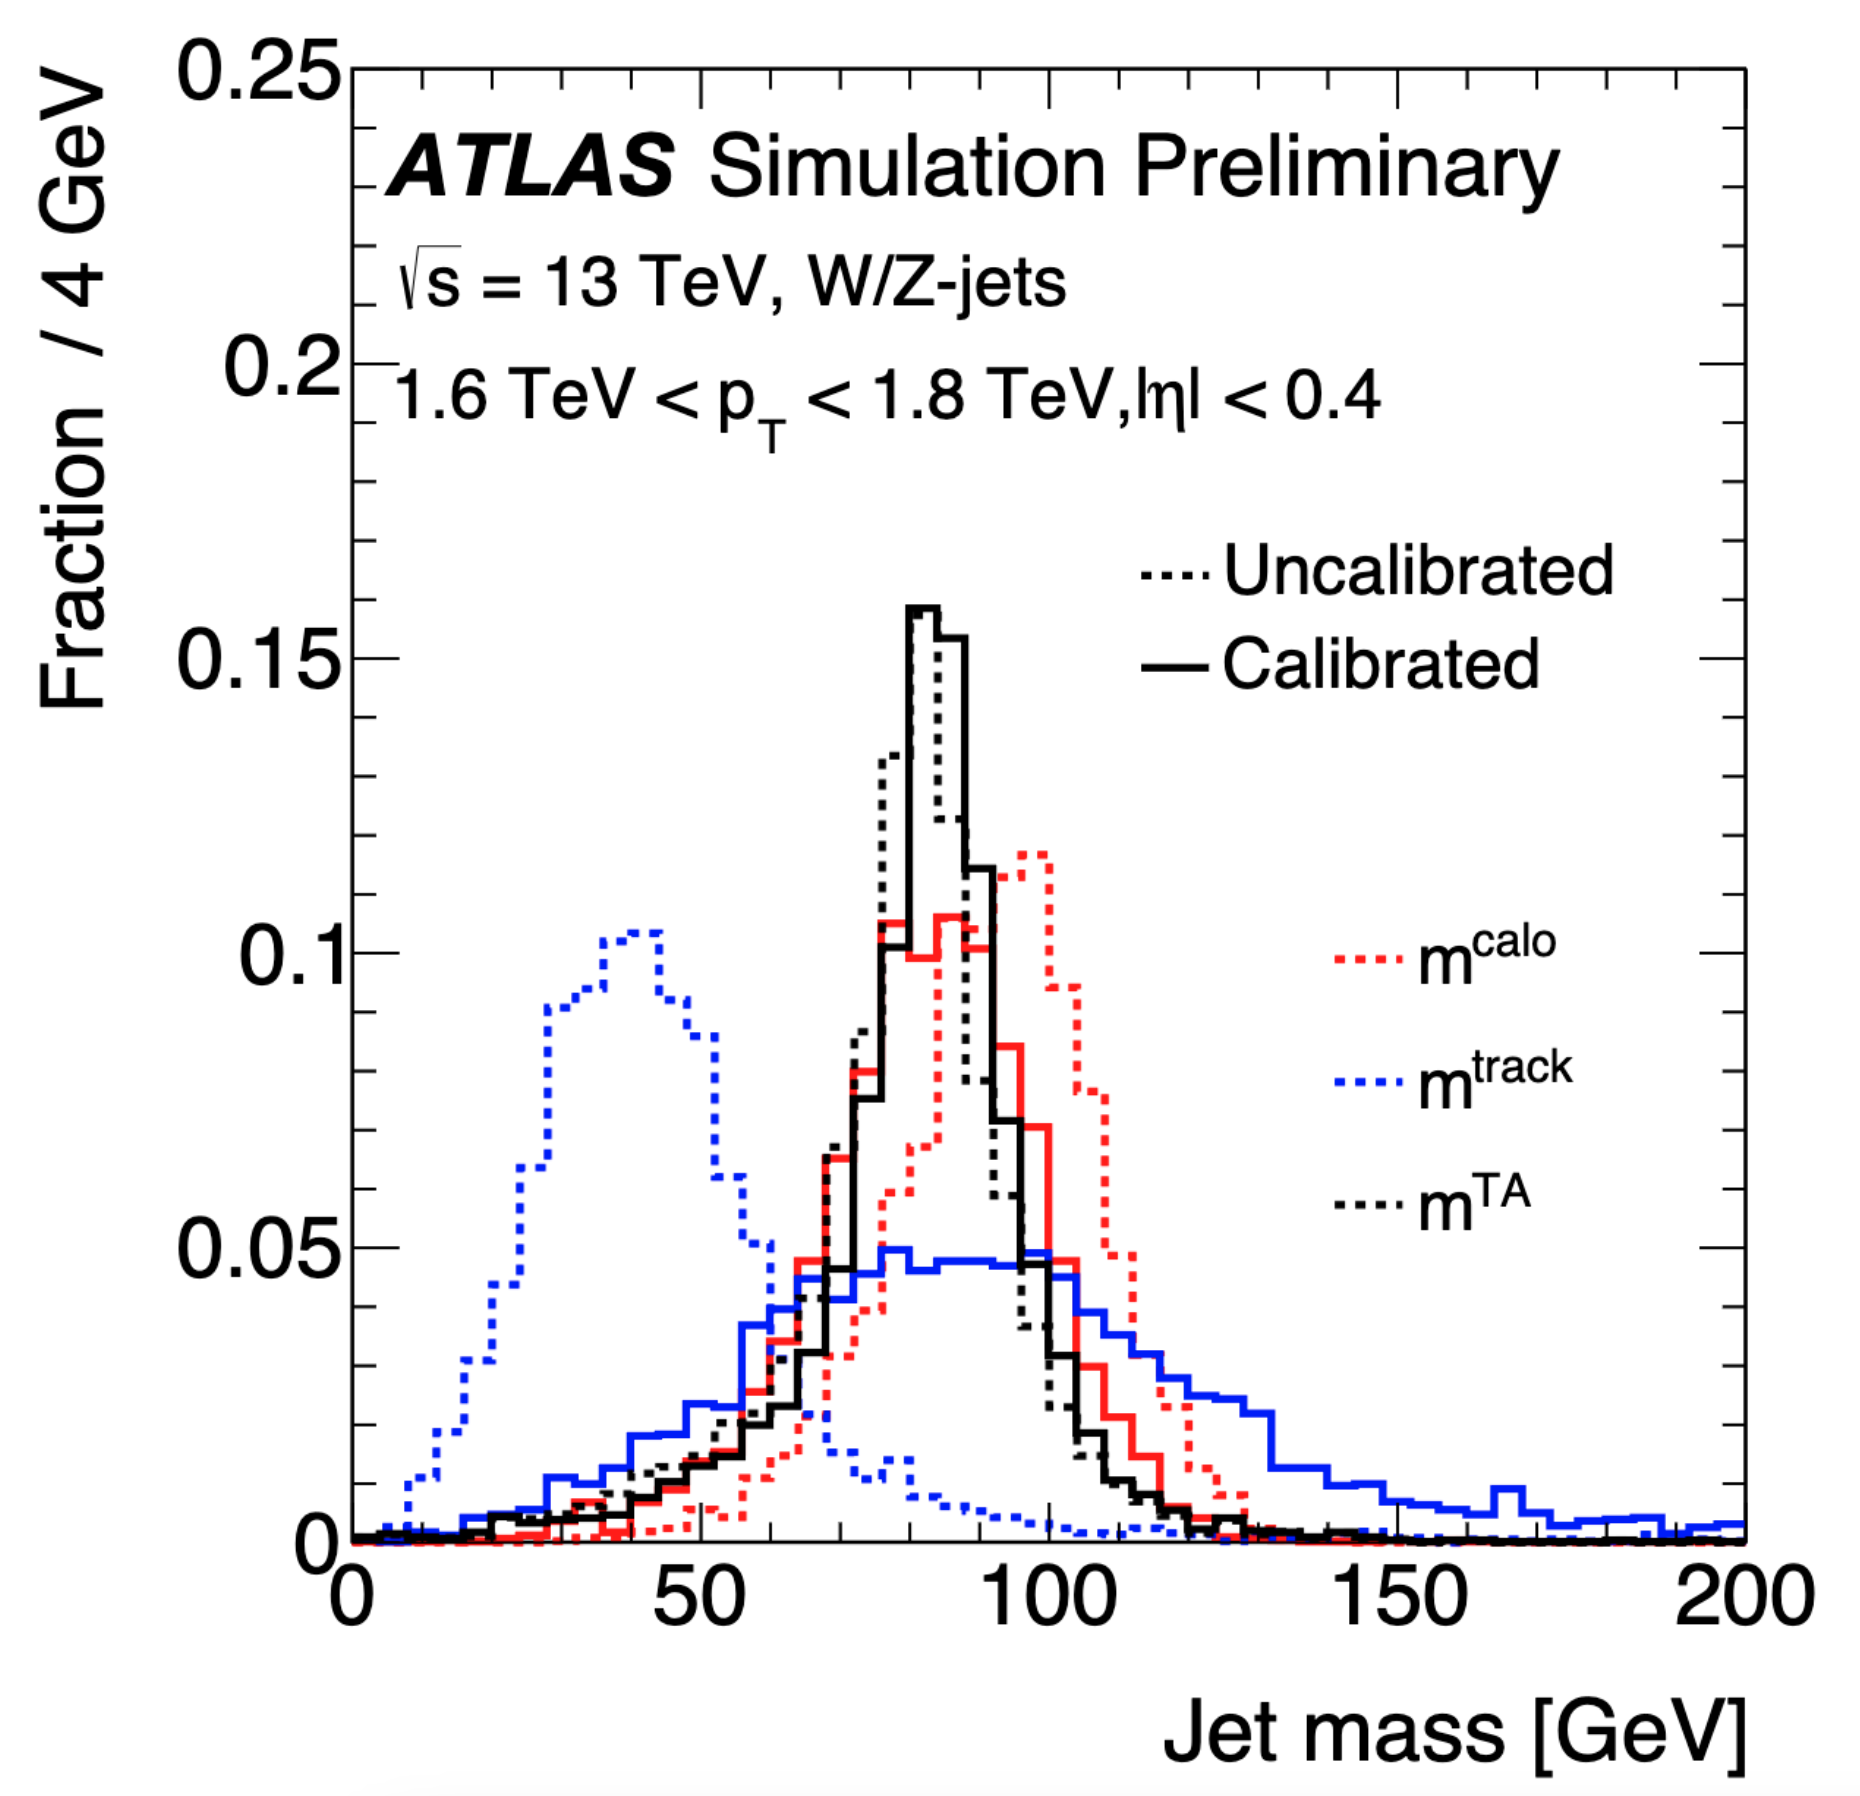
\includegraphics[width=.5\textwidth]{combined_mass_large_R}
  \caption[]{Improvement for track-assisted mass measurement compared to calorimeter and tracking information only. Adopted from \citep{ATLAS-CONF-2016-035} }
  \label{fig:combined_mass_large_R}
\end{figure}
